\documentclass{standalone}
\usepackage{tikz}
\usepackage{xcolor}

\usetikzlibrary{shapes,arrows}
\begin{document}
  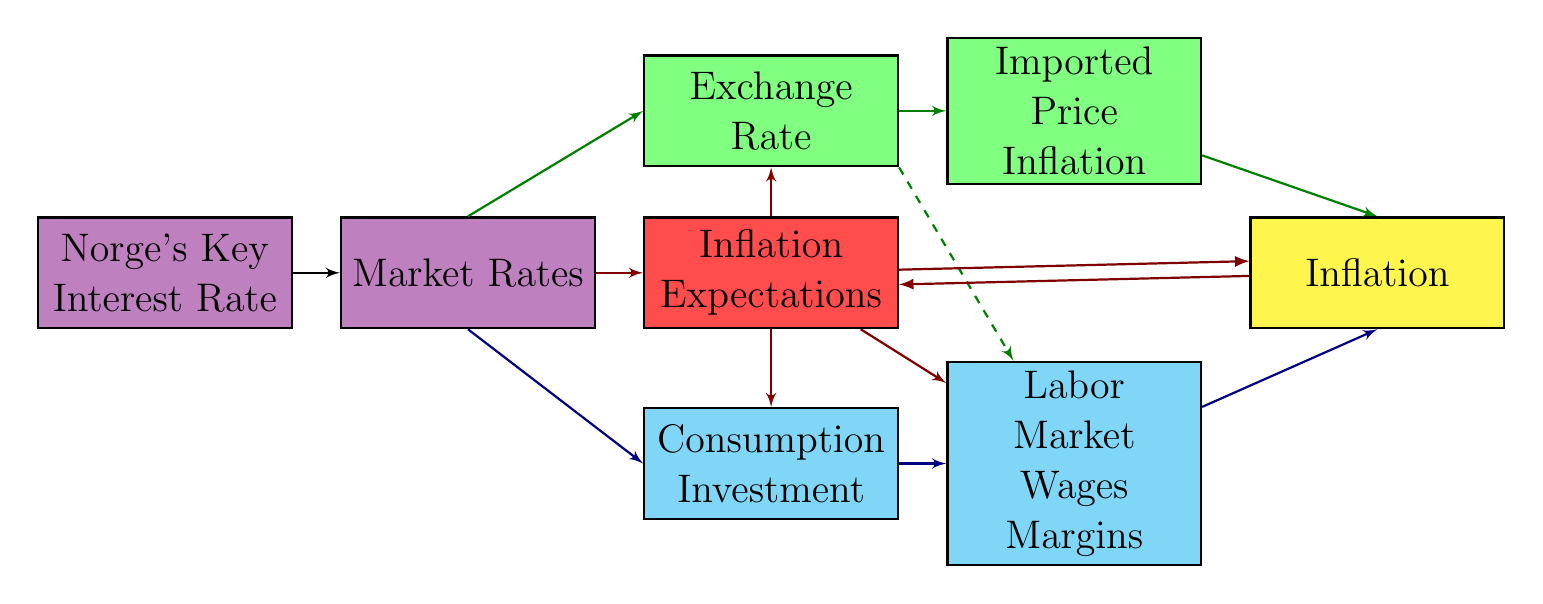
\begin{tikzpicture}[auto,
    %decision/.style={diamond, draw=black, thick, fill=white,
    %text width=8em, text badly centered,
    %inner sep=1pt, font=\sffamily\small},
    block_center/.style ={rectangle, draw=black, thick, fill=white,
      text width=8.5em, text centered, font=\Large,
      minimum height=4em},
      line/.style ={draw, thick, -latex', shorten >=0pt}]
    % outlining the flowchart using the PGF/TikZ matrix funtion
    \matrix [column sep=6mm,row sep=4mm] {
      % enrollment - row 1
      & &
      \node [block_center, fill=green!50] (excRate) {Exchange Rate}; &
      \node [block_center, fill=green!50] (impPrInf) {Imported Price Inflation}; & \\
      % enrollment - row 2
      \node [block_center, fill=violet!50] (keyRate) {Norge's Key Interest Rate}; &
      \node [block_center, fill=violet!50] (mrkRate) {Market Rates}; &
      \node [block_center, fill=red!70] (infExp) {Inflation Expectations}; &
      & \node [block_center, fill=yellow!70] (inf) {Inflation}; \\
      % enrollment - row 3
      & & \node [block_center, fill=cyan!50] (consInv) {Consumption Investment}; & 
      \node[block_center, fill=cyan!50] (lbrMrktMar) {Labor Market Wages Margins}; & \\
    };% end matrix
    % connecting nodes with paths
    \begin{scope}[every path/.style=line]
      \path [green!50!black] (excRate) -- (impPrInf);
      \path (keyRate) -- (mrkRate);
      \path [red!50!black] (mrkRate) -- (infExp);
      \path [red!50!black] (infExp) -- (consInv);
      \path [blue!50!black] (consInv) -- (lbrMrktMar);
      \path [red!50!black] (infExp) -- (excRate);
      \path [red!50!black] (infExp) -- (lbrMrktMar);
      \path [green!50!black] (mrkRate.north) -- (excRate.west);
      \path [blue!50!black] (mrkRate.south) -- (consInv.west);
      \path [dashed, green!50!black] (excRate.south east) -- (lbrMrktMar);
      \path [green!50!black] (impPrInf) -- (inf.north);
      \path [blue!50!black] (lbrMrktMar) -- (inf.south);
      \path [>=latex,->, red!50!black] ([yshift= 20pt]infExp) -- ([yshift= 20pt]inf);
      \path [>=latex,->, red!50!black] ([yshift= -20pt]inf) -- ([yshift= -20pt]infExp);      
    \end{scope}
  \end{tikzpicture}
\end{document}